\documentclass[a4paper,12pt]{article}

\usepackage[utf8]{inputenc}
\usepackage{geometry}
\usepackage{graphicx}
\usepackage{amsmath}
\usepackage{hyperref}

\geometry{margin=1in}

\title{Algorithm PA3 report}
\author{Ivan Chang}
\date{\today}

% Language and font packages
% \usepackage{ctex} % Chinese support

% Pseudocode and algorithm packages
\usepackage{algorithm2e} % Advanced algorithm writing
\usepackage{algpseudocode} % Pseudocode environment for algorithms

% Fancy style packages
\usepackage{fancyhdr} % Custom headers/footers
\usepackage{color} % Color support
\usepackage{xcolor} % Extended color support
\usepackage{tcolorbox} % Colored boxes
\usepackage{framed} % Framed environments

% Math and symbol packages
\usepackage{amsfonts}
\usepackage{amssymb}
\usepackage{mathtools}

% Table and figure packages
\usepackage{booktabs} % Professional tables
\usepackage{multirow} % Multi-row tables
\usepackage{caption} % Custom captions
\usepackage{subcaption} % Subfigures

% Miscellaneous
\usepackage{enumitem} % Custom lists
\usepackage{listings} % Code listings
\usepackage{tikz} % Drawing diagrams
\usepackage{pgfplots} % For plotting graphs
\usepackage{float}

\begin{document}

\maketitle

\section{Data Structure}

To efficiently handle the 3D Global Routing problem, we implemented several key data structures designed to optimize memory usage and access speed.
\subsection{Graph Construction}
The routing grid is abstracted into a graph $G = (V, E)$ stored as an adjacency list (\texttt{std::vector<std::vector<Edge>>}).
\begin{itemize}
    \item \textbf{Vertices ($V$)}: Each GCell corresponds to a vertex.
    \item \textbf{Edges ($E$)}: Edges connect adjacent GCells in the x, y (planar) and z (via) directions.
    \item \textbf{Edge Weights}: Each edge stores a \texttt{baseCost}, which represents the physical wirelength ($W_j$, $H_i$) or the via cost ($WL_{via}$).
\end{itemize}

\subsection{Net and Coordinates}
Nets are stored as a struct containing the net name and two \texttt{Coord3D} pins. The \texttt{Coord3D} structure simply holds $\{layer, col, row\}$.

\section{Cost Function}

The core of the global router relies on a dynamic cost function that penalizes congestion. The cost of traversing an edge $e(u, v)$ is defined as the physical length plus the congestion penalty of the target vertex $v$.

\subsection{Vertex Cost Formulation}
In \texttt{router.cpp}, the function \texttt{computeVertexCost} calculates the penalty for occupying a GCell based on current overflow. The cost is exponential to heavily discourage using overflowing cells.

Let $D_v$ be the demand and $C_v$ be the capacity of vertex $v$. The overflow is $O_v = \max(0, D_v - C_v)$. The base vertex cost is:
\begin{equation}
    Cost_{base}(v) = \alpha \times (2^{O_v} - 1) + \mathbb{I}(O_v > 0) \times P_{overflow}
\end{equation}
Where:
\begin{itemize}
    \item $\alpha = 1000$ (Scaling factor).
    \item $P_{overflow} = 100,000$ (A large fixed penalty added if any overflow exists).
    \item The overflow $O_v$ is clamped at 20 to prevent integer overflow.
\end{itemize}

\subsection{History Cost (Negotiation)}
To resolve contention between nets that repeatedly compete for the same resources, we employ a history-based cost.
\begin{equation}
    Cost_{total}(v) = Cost_{base}(v) + \beta \times h_v
\end{equation}
Where:
\begin{itemize}
    \item $h_v$ is the history count, incremented by 1 in every iteration where GCell $v$ is overfull.
    \item $\beta = 1000$ is the history penalty factor.
\end{itemize}

This ensures that if a cell remains congested over many iterations, its cost rises permanently, forcing nets to explore alternative, longer paths.

\section{Routing Strategy}

We implemented a Negotiation-based Rip-up and Reroute (RRR) strategy utilizing the A* search algorithm.

\subsection{A* Search Algorithm}
Pathfinding is performed using A* search.
\begin{itemize}
    \item \textbf{Heuristic ($h(n)$)}: We use the 3D Manhattan distance between the current GCell and the target pin. This is admissible and consistent, ensuring optimal pathfinding relative to the current edge weights.
    \item \textbf{Cost ($g(n)$)}: The accumulated cost from the source.
    \item \textbf{Weight Calculation}: In the relaxation step, the weight to move from $u$ to $v$ is $EdgeLength(u,v) + Cost_{total}(v)$.
\end{itemize}
This allows the router to balance wirelength minimization (via edge lengths) and congestion avoidance (via vertex costs).

\subsection{Rip-up and Reroute (RRR) Workflow}
The routing process proceeds iteratively:
\begin{enumerate}
    \item \textbf{Initial Routing}: Route all nets sequentially using A* on an empty grid (considering only physical capacity constraints).
    \item \textbf{Iterative Refinement}:
    \begin{itemize}
        \item Calculate total overflow. If 0, the solution is valid and we terminate.
        \item Update history costs for all currently overfull GCells.
        \item \textbf{Net Selection}: Identify nets passing through overflowed GCells.
        \item \textbf{Ordering}: Shuffle the selected nets randomly, then sort them based on the number of overflow hits (nets causing the most congestion are routed first).
        \item \textbf{Reroute}: For each selected net:
        \begin{enumerate}
            \item \textbf{Rip-up}: Remove the net's demand from the grid.
            \item \textbf{Update Graph}: Recalculate vertex costs with the updated demand and history.
            \item \textbf{Route}: Run A* to find a new path.
            \item \textbf{Commit}: Add the new path's demand to the grid.
        \end{enumerate}
    \end{itemize}
\end{enumerate}

\subsection{Stagnation Control}
To prevent the algorithm from getting stuck in local minima, we track a stagnation counter. If the total overflow does not decrease for 200 consecutive iterations (\texttt{stagcnt >= 200}), we force a full reroute of \textit{all} nets, not just the congested ones, to perturb the system significantly.

\section{Results and Analysis}

\subsection{Experimental Results}
The router was tested on the provided benchmarks. Below is a summary of the performance metrics.

% FILL IN THE TABLE BELOW WITH YOUR ACTUAL OUTPUT DATA
\begin{figure}[H]
    \centering
    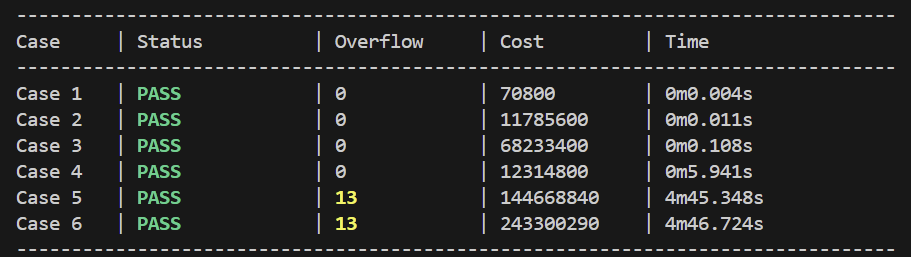
\includegraphics[width=0.8\textwidth]{result.png}
    \caption{Routing Results Summary}
    \label{fig:results}
\end{figure}
 

\subsection{Analysis}
\begin{itemize}
    \item \textbf{Effectiveness of History Cost}: The inclusion of the history variable $h_v$ was critical. In early iterations, nets oscillated between two equally congested paths. The history cost broke this symmetry by permanently penalizing the frequently contended nodes.
    \item \textbf{Exponential Penalty}: Using $2^{overflow}$ provided a strong gradient. It allowed the router to distinguish between "slightly congested" (overflow 1) and "heavily congested" (overflow 5), guiding paths toward the former if necessary.
    \item \textbf{Runtime vs. Quality}: The A* heuristic significantly sped up the search compared to Dijkstra for it only explores promising paths. However, the overall runtime is still dominated by the number of iterations needed to resolve congestion.
\end{itemize}
\end{document}